\chapter{Simulation and Reconstruction}\label{chap:SimReco}
In order to perform physics analyses, signals collected by the ATLAS detector are reconstructed into meaningful physics objects. This chapter presents the concept of \emph{Monte-Carlo} simulation. It is introduced as a method to estimate predicted rates of specific SM and BSM processes. Also, a description of the reconstruction and identification of physics objects is provided in this chapter. 

\section{Event simulation}\label{sec:simulation}
The theoretical understanding of high-energy physics processes are tested by making comparisons of experimental data with theoretical predictions. These comparisons usually utilise simulated collision events that can be analysed. Production of simulated data requires the theoretical modelling of many aspects of \protonproton collisions and their resulting products. The simulation process is separated into collision event generation and detector simulation.

The simulation of collision events is split into two main parts: firstly, the simulation of the matrix element process, and then the resulting parton shower and hadronisation process. A predicted cross-section is calculated by integrating the matrix element over the phase space of the final state. Detailed knowledge of the distribution of partons in each proton is required in the form of \emph{parton distribution functions} (PDFs), to correctly predict the cross-section and kinematics of a process. The PDFs give the probability for a parton of a given type to be found with some fraction of the proton's initial momentum. The matrix element calculations are performed at fixed-order in perturbation theory. Therefore, the production of quarks and gluons beyond the order of the calculation is required to be handled separately. 

High-energy outgoing quarks and gluons emit QCD radiation as the scale of the process evolves. The emission of QCD radiation is in the form of \emph{parton showers}, which are higher-order emissions of additional gluons, or the forming of quarks via the splitting of gluons. The production of such processes are modelled by the \emph{DGLAP equations}~\cite{Dokshitzer77,Gribov72,Altarelli77}. The DGLAP equations scale the probabilities for a given type of parton to split into additional partons as a function of energy until the partonic energy scale has reached about \SI{1}{\giga\electronvolt}. Below this energy threshold, the lone quarks and gluons form colourless objects (mesons and baryons) in a process called \emph{hadronisation}.  This process is simulated with non-perturbative models~\cite{Andersson1983,Webber1984}. Finally, decays of short-lived particles ($c\tau<\SI{10}{\milli\metre}$), who do not have a long enough lifetime to interact with the ATLAS detector are simulated at this stage. 

Several different simulation groups specialise in matrix element simulations and parton shower simulations. A dedicated combination package handles a careful matching of the simulation of the matrix element, and parton shower simulations, which is then used to produce individual datasets of simulated events. Additionally, the pileup interactions between other protons in the beam are also overlaid on the produced hard scatter simulated events to produce a full description of the colliding beams. 

The simulation of the interactions of the particles produced in collisions is handled by the \textsc{Geant4} simulation software~\cite{Geant1,Geant2,Geant3}, which provides a detailed computer model of the ATLAS detector materials, geometry and also includes the wiring in the detector. The output of the detector simulation is treated the same as measurements of real data events made by the detector to preserve the compatibility between the simulated and real reconstructed data. 

Full simulation of interactions with the detector can be computationally intensive and results in a significant use of resources for the experiment. The analysis presented in this thesis in~\cref{chap:intro} requires multiple samples of large numbers of events to be produced to be sensitive to new physics phenomena. The analysis described in this thesis introduces an alternative method that does not rely on the production of large simulated datasets which require full detector simulation, drastically reducing the strain on available resources. Simulation of objects at generator level before detector simulation is referred to as \emph{truth}-level, whereas objects produced after the detector simulation is referred to as \emph{reconstructed (reco)}-level.

\section{Reconstruction of physics objects}\label{sec:reconstruction}
The reconstruction, identification and isolation of the types of physics objects used in the thesis are described in this section. 

\subsection{Tracks and vertex reconstruction}\label{sec:reconstruction:tracks}
The identification of tracks are essential in the reconstruction of physics objects and in identifying interaction vertices. Track reconstruction aims to describe the trajectory of a particle through the inner detector. Additionally, the muon tracks are also reconstructed in the muon spectrometer described in ~\cref{sec:method:MS}. A series of sequential algorithms are used to reconstruct tracks from the inner detector readout~\cite{ATLAS:tracking}. 

Measurements from the pixel and SCT layers are reconstructed into \emph{hits}, defined by three-dimensional space points. Hits from either side of the modules are required to form both coordinate in the SCT, and timing information from the TRT is used to construct drift circles. \emph{Track seeds} are formed from three hits in the pixel detector and the first layer of the SCT. These track seeds are extended into the outermost layers of the SCT to give \emph{track candidates}, which are then fit to the hits produced using a Kalman-filter~\cite{ATLAS:tracking,ATLAS:Kalman}. The Kalman-filter takes into account the scattering of tracks by materials of the detector. Poor quality tracks are rejected by applying a score based on the $\chi^2$ of the fit and the number of missing hits in active detector layers. Ambiguities in space points corresponding to multiple tracks are also removed by selecting the highest-scoring tracks. The remaining tracks are then extended to the TRT to provide many more additional hits. Final reconstructed tracks are then formed by fitting to all the detector components simultaneously. 

A subsequent algorithm extending inwards from hits in the TRT is used to find track segments that were missed by the previous method. Tracks segments in the TRT not associated with tracks in the first algorithm are extrapolated inwards to hits in the SCT and pixel detectors. An example of such track segments detected in the inner detector is shown in \cref{fig:method:tracking-outside-in}. A similar ambiguity-resolving criteria as the first algorithm based on the $\chi^2$ is also applied. 
\begin{figure}[]
    \centering
    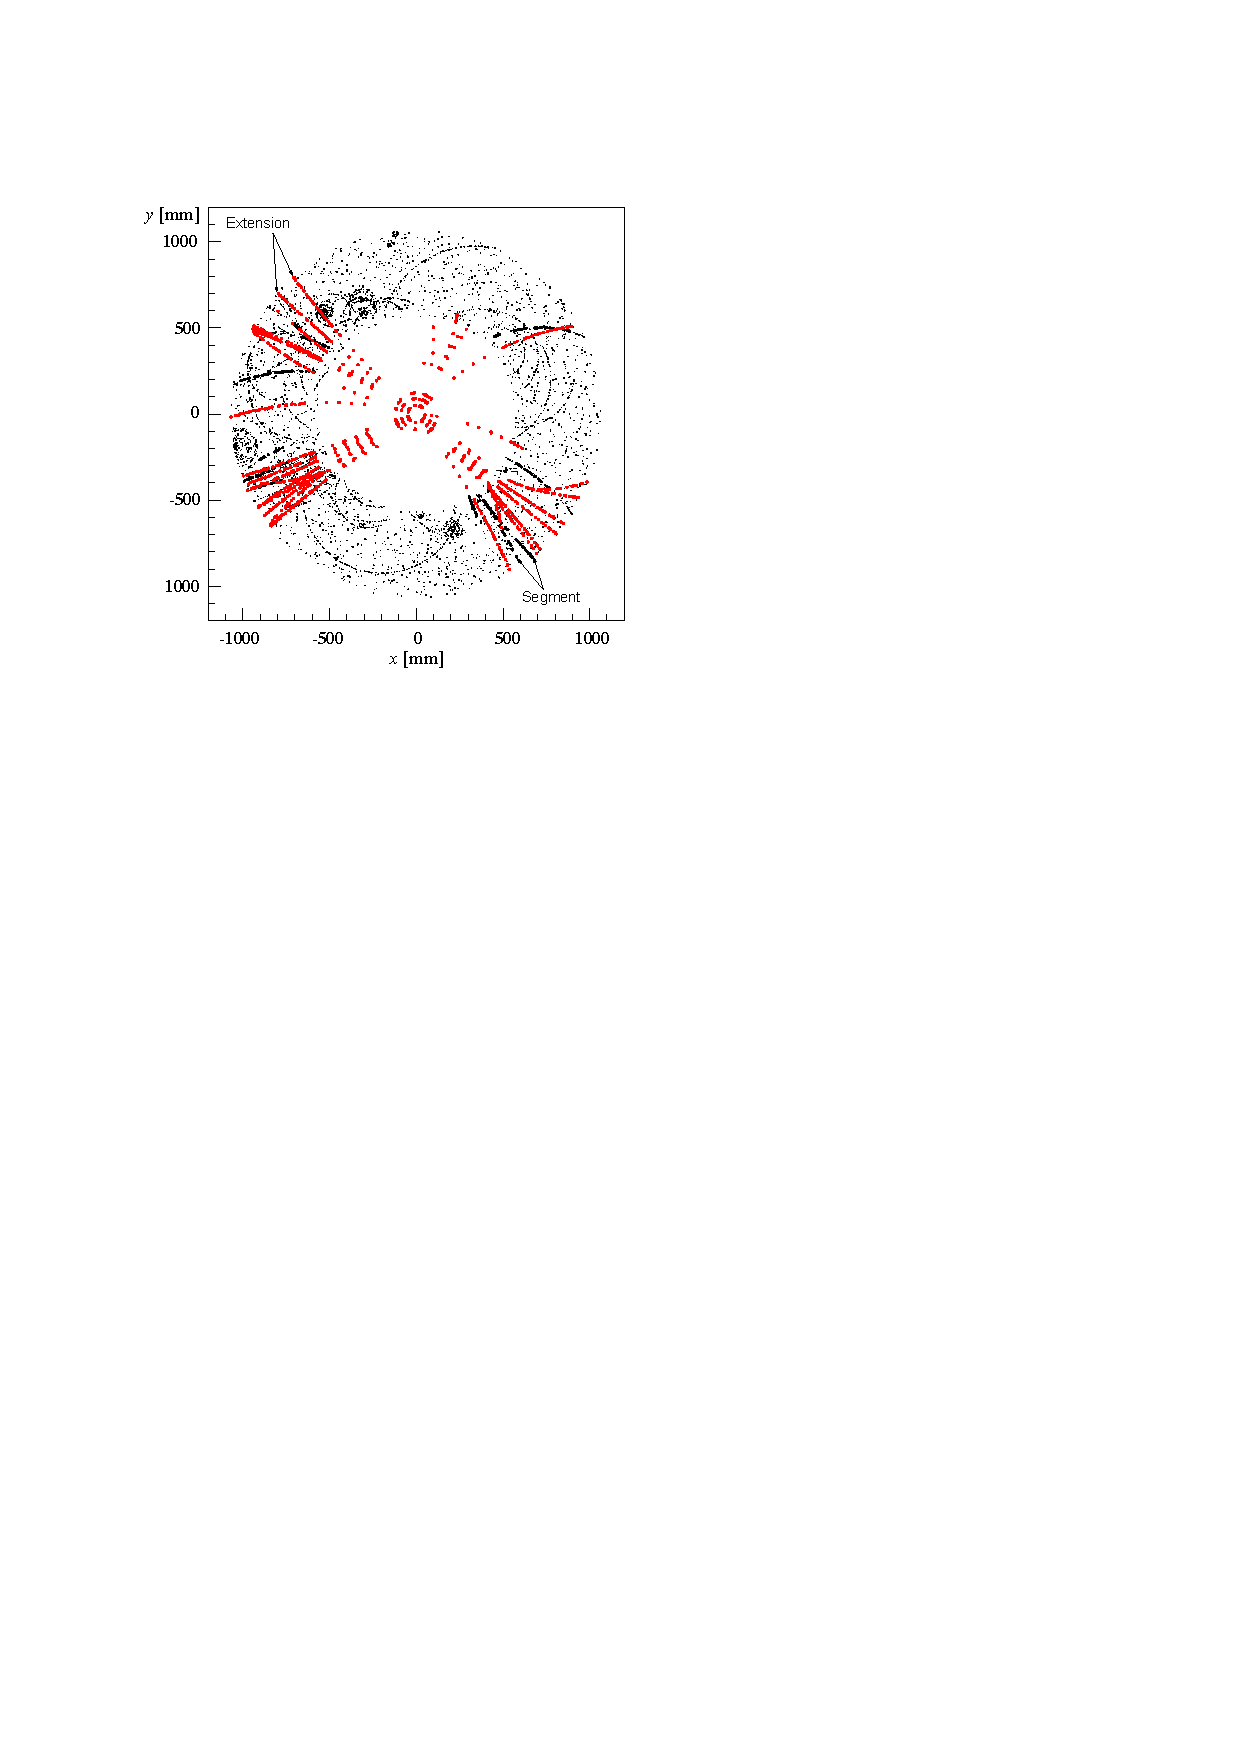
\includegraphics[width=\mediumfigwidth]{images/tracking-outside-in.pdf}
    \caption[Track finding for a simulated \ttbar event]{Track finding for a simulated \ttbar event.
    Hits are indicated by small black dots in the transverse plane.
    Red dots show hits in associated with tracks that originate from following the SpacePoint seeded tracks into the TRT
    Black circles indicate hits that form track segments in the TRT , which builds the start point of the back tracking application~\cite{ATLAS:tracking}.}
    \label{fig:method:tracking-outside-in}
\end{figure}

There are multiple \protonproton collisions per bunch crossing at the LHC due to its high instantaneous luminosity. \cref{fig:method:ATLAS-pileup} shows the distribution of the number of interactions per bunch crossing. The vertex of an interaction indicates the location at which the physical process has occurred. Once all tracks have been fitted, vertex finder algorithms are used to assign the tracks to their corresponding vertex. Reconstructed vertices are required to have at least two tracks associated with them. The primary vertex is determined as the \protonproton interaction vertex with the highest sum of the transverse momentum of its associated tracks, indicating it as the vertex at which the hard scattering is most likely to have originated. The other \protonproton interactions are referred to as \emph{pileup}. Vertex reconstruction is essential in removing objects that originate from pileup interactions and for measurements of properties of long-lived particles. 
\begin{figure}[]
    \centering
    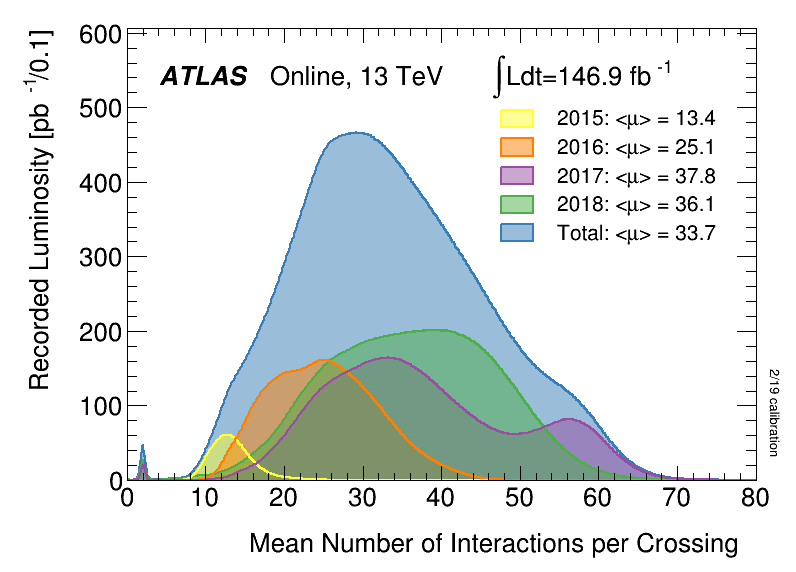
\includegraphics[width=\mediumfigwidth]{images/mu_2015_2018.png}
    \caption[Distribution of number of interactions per \protonproton bunch crossing in ATLAS for the 2015+2018 data-taking period]{Distribution of number of interactions per \protonproton bunch crossing in ATLAS for the 2015+2018 data-taking period~\cite{ATLAS:lumiPlots}.}
    \label{fig:method:ATLAS-pileup}
\end{figure}

\subsection{Electrons}\label{sec:reconstruction:electrons}
Electrons and positrons have the same experimental signature in the EM calorimeter. They are only distinguishable due to the difference in the curvature of their tracks in the ID. In this thesis, positrons will also be referred to as electrons.   

Electron reconstruction involves using track information from the ID with calorimeter information from the EM calorimeter and the pattern of electrons transition radiation as they pass through the TRT.

\subsubsection{Electron reconstruction}
The measurement of an electron signature can be characterised by a localised energy deposit (cluster) in the EM calorimeter and charged tracks in the ID that are matched to the cluster that forms the final electron candidate. Electrons lose energy when traversing the ID due to bremsstrahlung, resulting in radiated photons. These photons can then be converted into electrons which then undergo further bremsstrahlung. Most of the energy of the electrons and photons are deposited within the EM calorimeter as they are collimated. This effect can result in multiple tracks being matched to the same electromagnetic cluster. 

A sliding window algorithm~\cite{slidingwindow} is utilised to search for localised clusters in the EM calorimeter. The EM calorimeter is divided into an $\eta \times \phi$ matrix. Initially, windows which correspond to a $3 \times 5$ granularity in the second layer of the EM calorimeter ($0.025 \times 0.025$) are formed. The matrix is searched using the windows for energy deposits with $E_T > \SI{2.5}{\giga\electronvolt}$. The identified clusters are used as seeds to match corresponding reconstructed tracks in the ID. The Gaussian Sum Filter (GSF) method~\cite{ATLAS:CONF-2012-047} is used to refit the reconstructed tracks, which takes into account the effects bremsstrahlung energy loss characteristic to electrons. If no suitable GSF-track is matched to an EM calorimeter cluster, the cluster is labelled as originating from photons.  After matching the track, the cluster is then rebuilt by summing the energies of all the cells within the $3 \times 7$ ($5 \times 5$) window in the barrel (end-cap).

The efficiency of the sliding window algorithm to reconstruct EM-cluster candidates in the EM calorimeter varies as a function of $\eta$ and $E_T$. \cref{fig:method:slidingwindow-reco} shows that the reconstruction efficiency as a function of $E_T$, ranging from 65\% at $E_T = \SI{4.5}{\giga\electronvolt}$ to more than 99\% above $E_T = \SI{15}{\giga\electronvolt}$. This efficiency is determined from simulation.

\begin{figure}[]
    \centering
    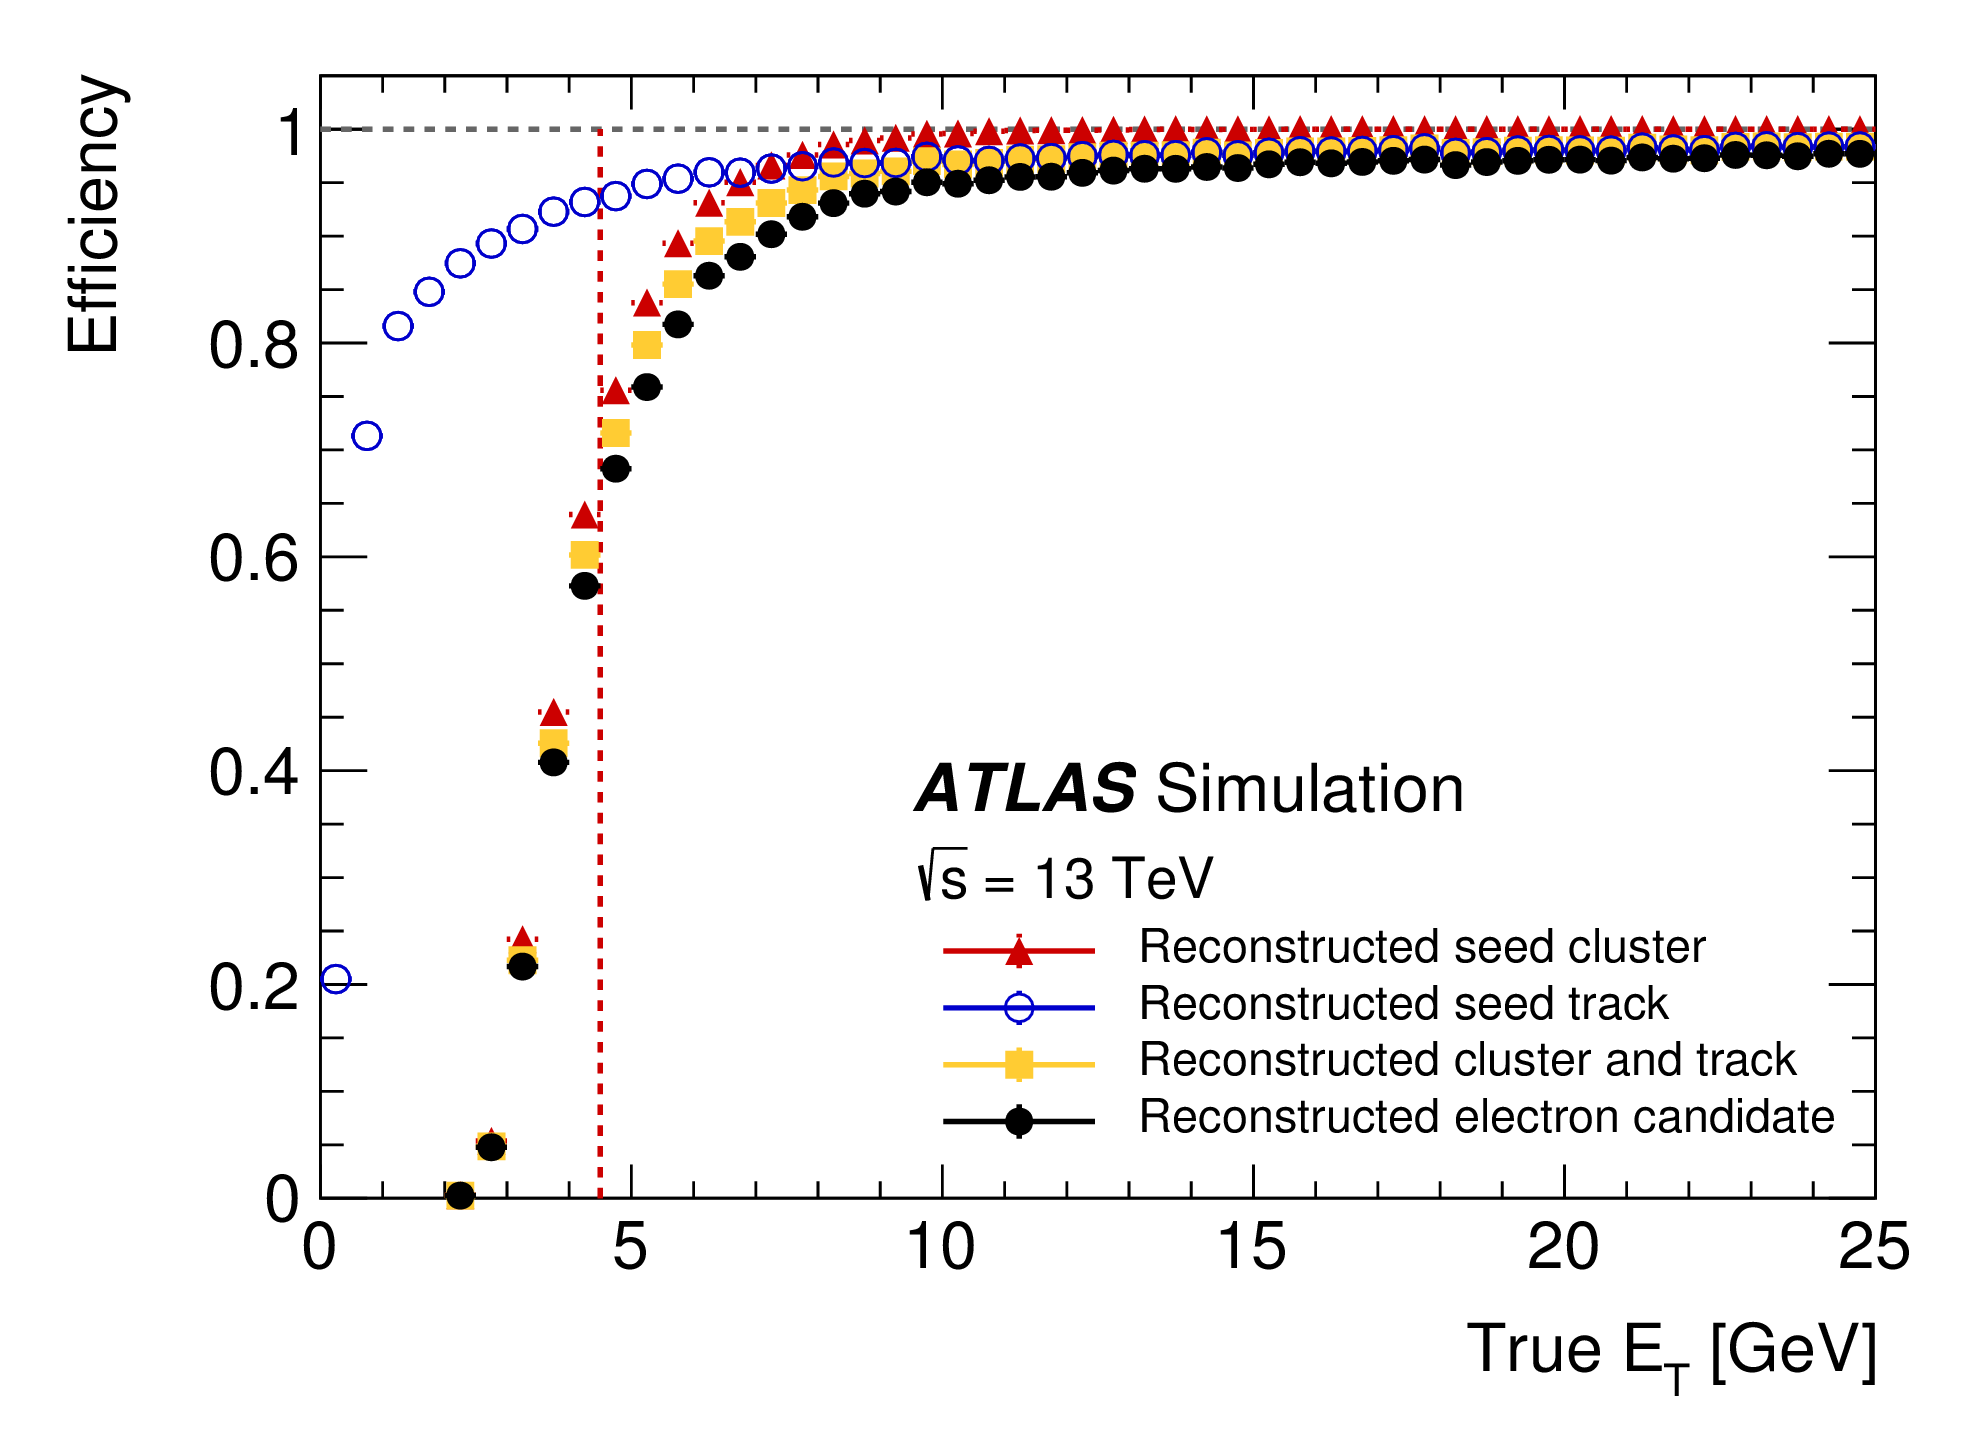
\includegraphics[width=\mediumfigwidth]{images/2015_2016_recoeff.png}
    \caption[Total reconstruction energy for simulated electrons using the sliding window algorithm]{The total reconstruction efficiency for simulated electrons in a single-electron sample as a function of truth level transverse energy, $E_T$, for each step of electron candidate formation~\cite{slidingwindowreco}.}
    \label{fig:method:slidingwindow-reco}
\end{figure}

From 2017 a new clustering algorithm has been adopted based on topological clusters (topo-cluster)~\cite{Aad:2019tso}. The topological clusters allow for the recovery of low energy deposits from bremsstrahlung photons and associate them to the electron cluster, forming a \emph{supercluster}. ~\cref{fig:method:superclusterscheme} shows a diagram of this procedure. In contrast to the sliding window algorithm, the cell significance, $\zeta^{\mathrm{EM}}_{\mathrm{cell}}$, is responsible for the seeding in a topo-cluster and is defined as

\begin{equation}
    \zeta^{\mathrm{EM}}_{\mathrm{cell}} = \abs{\frac{E^{\mathrm{EM}}_{\mathrm{cell}}}{\sigma^{\mathrm{EM}}_{\mathrm{cell,noise}}}},
\end{equation}

where $\abs{E^{\mathrm{EM}}_{\mathrm{cell}}}$ is the absolute cell energy and $\sigma^{\mathrm{EM}}_{\mathrm{cell,noise}}$ is the expected cell noise. The clustering algorithm initially forms a \emph{proto-cluster} using a set of noise thresholds in which the first cell is required to have $\abs{E^{\mathrm{EM}}_{\mathrm{cell}}} \geq 4$. Then all immediate neighbouring cells with $\abs{E^{\mathrm{EM}}_{\mathrm{cell}}} \geq 2$ around the proto-cluster are added. Finally, cells with $\abs{E^{\mathrm{EM}}_{\mathrm{cell}}} \geq 0$ adjacent to the cells that were previously included are also added to the cluster. This formalism is known as the "4-2-0" topo-cluster reconstruction. A supercluster is built from a topo-cluster seed after satellite candidates, possibly emerging from bremsstrahlung radiation around a seed candidate, have been resolved. \cref{fig:method:screco} shows the efficiency for the different components of the supercluster-based reconstruction. The same track fitting method used in the sliding window algorithm is used to refit the reconstructed tracks.
\begin{figure}[h]
    \centering
    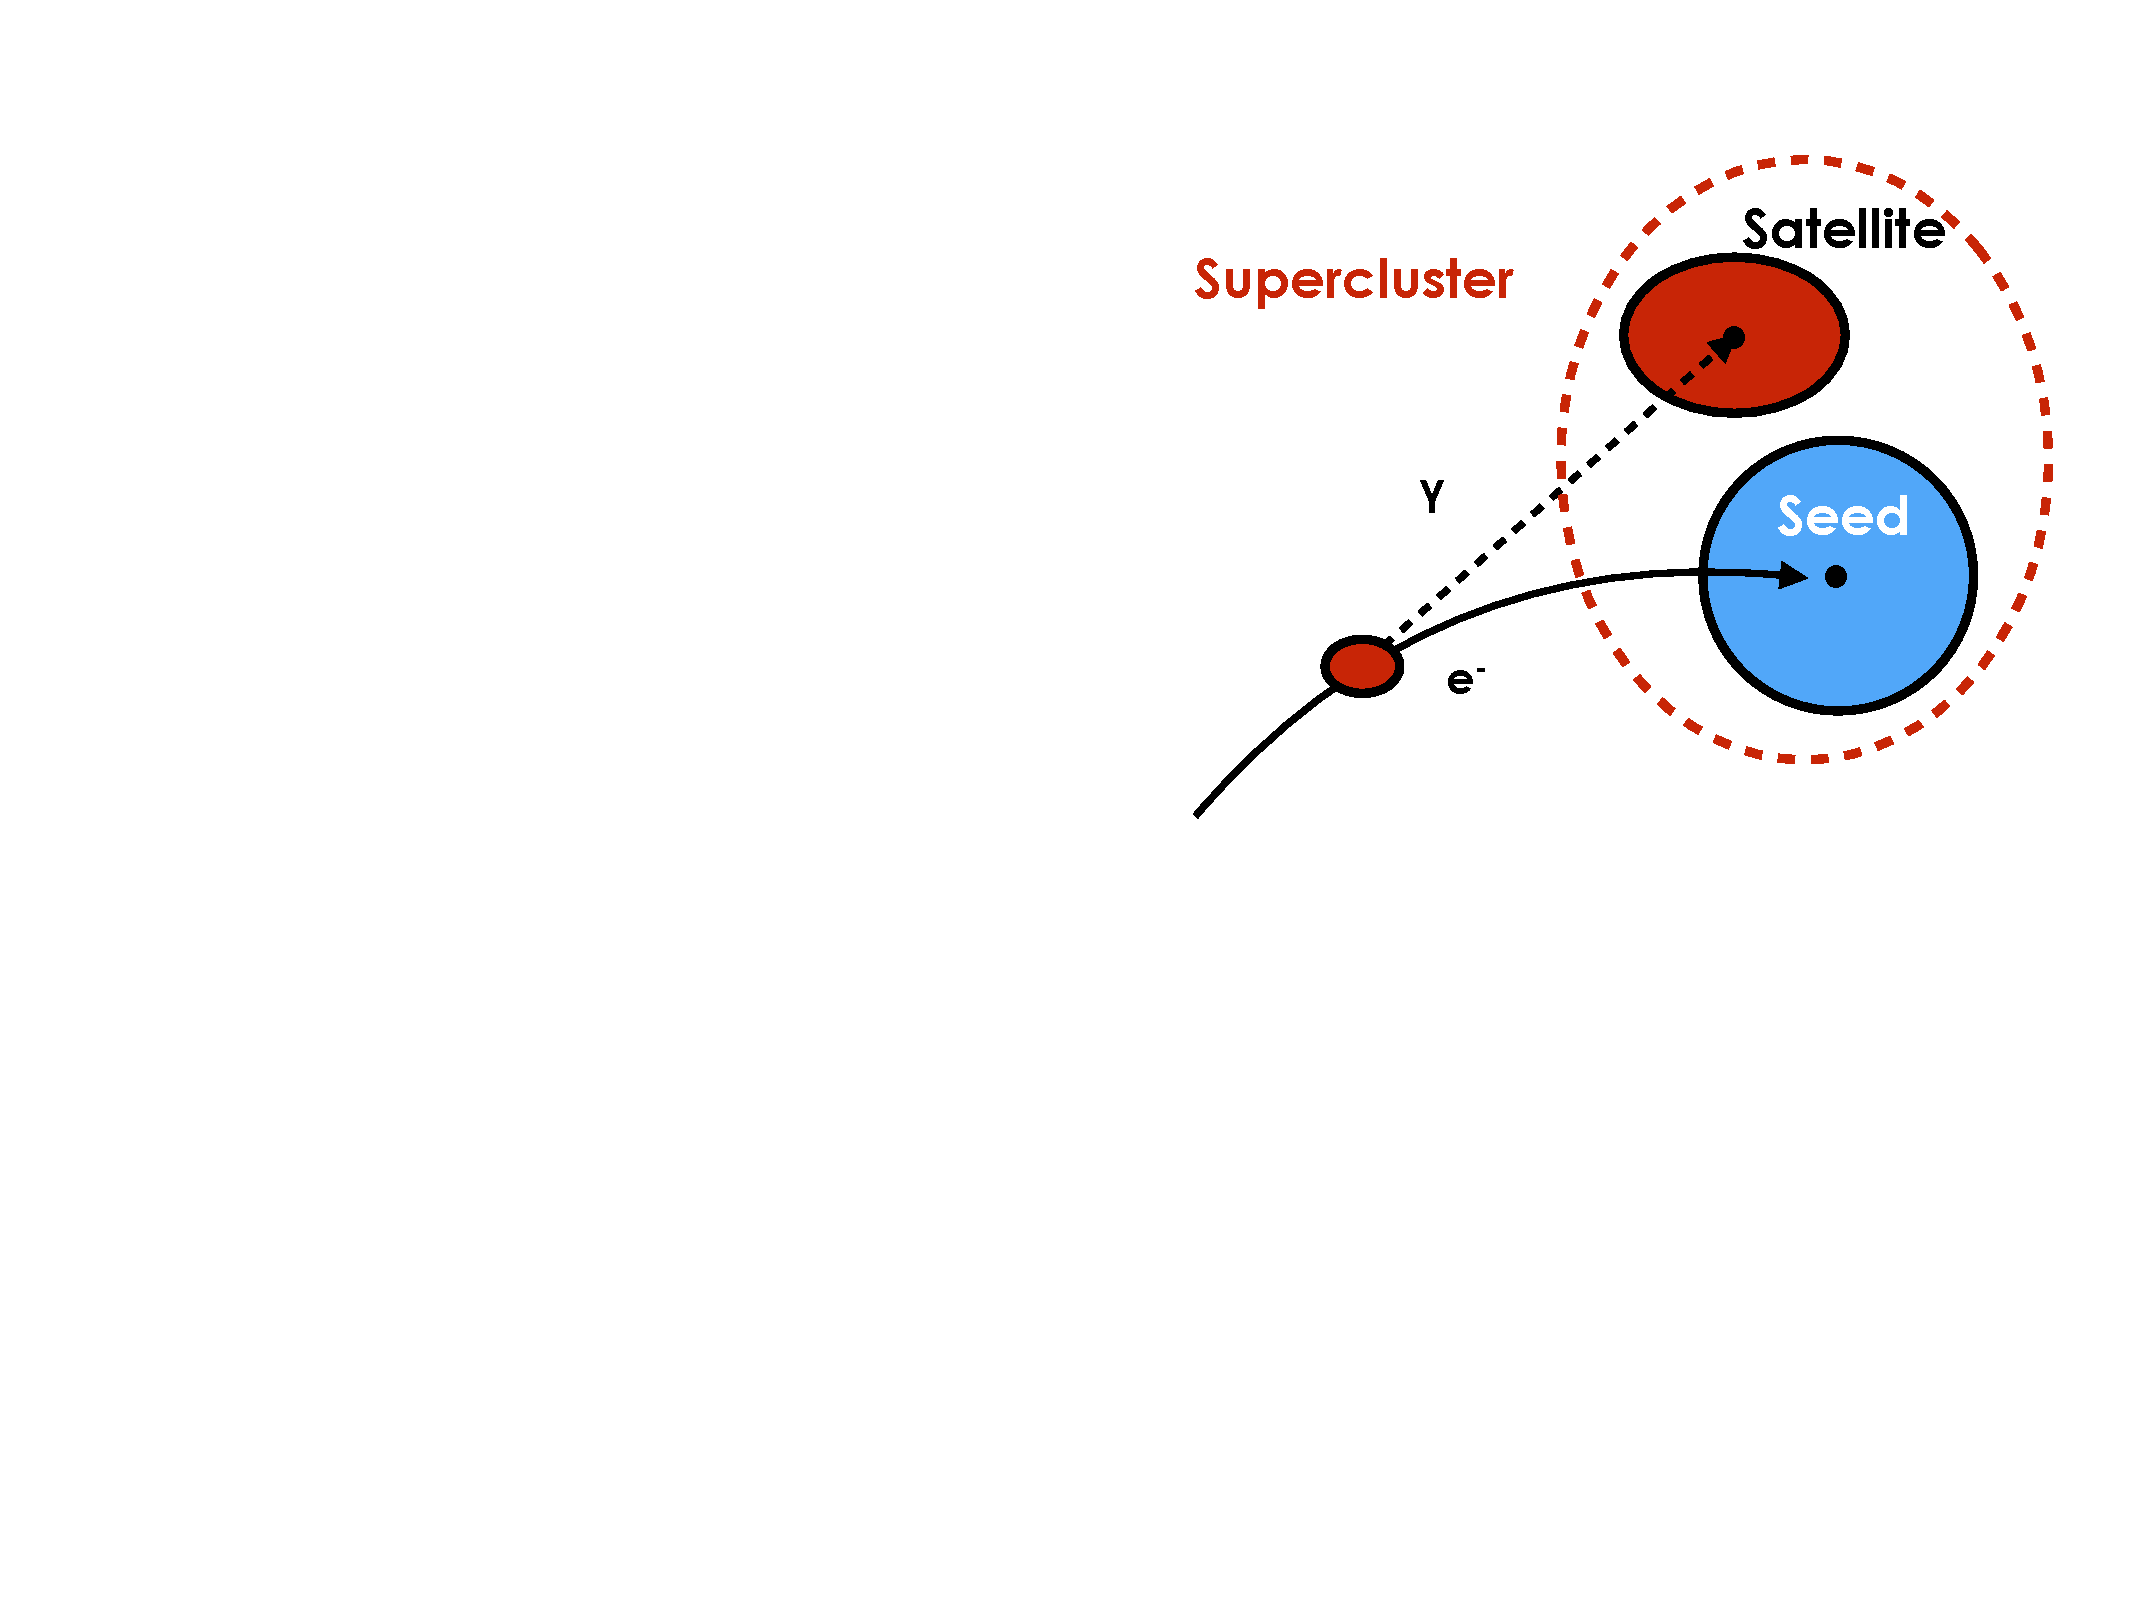
\includegraphics[width=\mediumfigwidth]{images/topo-cluster.pdf}
    \caption[Diagram of an example supercluster showing a seed electron cluster and a satellite photon cluster.]{Diagram of an example supercluster showing a seed electron cluster and a satellite photon cluster~\cite{ATL-PHYS-PUB-2017-022}.}
    \label{fig:method:superclusterscheme}
\end{figure}
\begin{figure}[h]
    \centering
    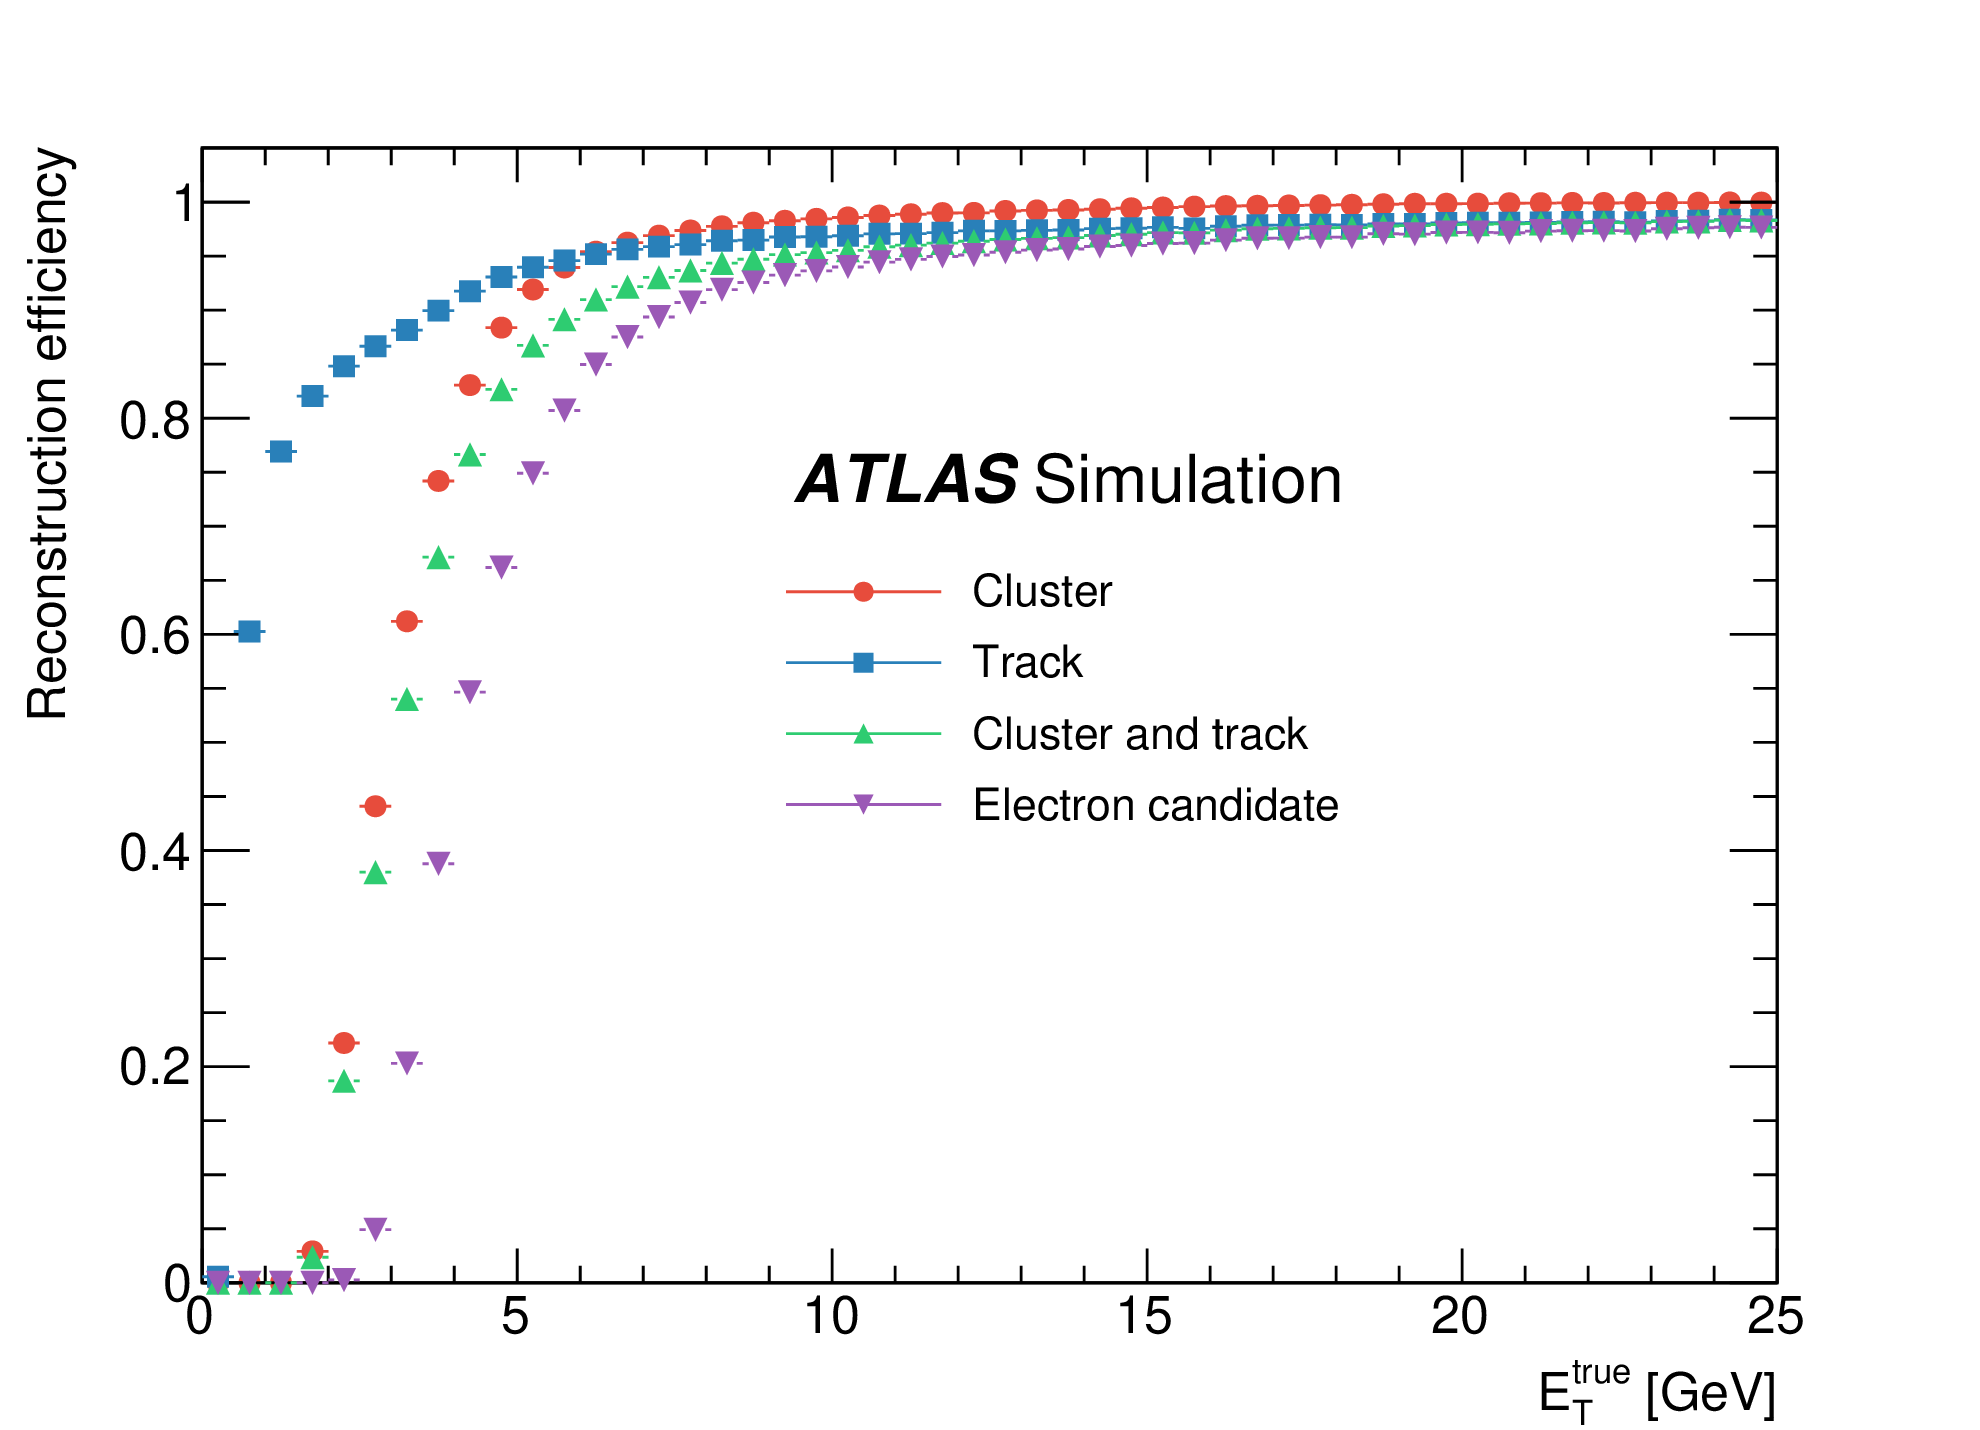
\includegraphics[width=\mediumfigwidth]{images/supercluster_reco.png}
    \caption[Supercluster-based cluster, track, cluster and track, and electron reconstruction efficiencies as a function of the generated electron $E_T$ ]{Supercluster-based cluster, track, cluster and track, and electron reconstruction efficiencies as a function of the generated electron $E_T$~\cite{Aad:2019tso}.}
    \label{fig:method:screco}
\end{figure}

The supercluster-based algorithm provides an improved energy resolution compared to the sliding window algorithm by collecting more energy deposits. The peak energy response $E_{calib}/E_{true}$ does not deviate by more than 0.5\% for the different particles, where $E_{true}$ is the energy of the particles before detector simulation and $E_{calib}$ is the calibrated reconstructed energy. The \emph{effective interquartile range} (IQE) compares the width (resolution) of the energy response and is used to quantify the performance of the supercluster algorithm compared to the sliding window algorithm. The IQE is given by
\begin{equation}
    IQE = \frac{Q_3 - Q_1}{1.349},
\end{equation}
where $Q_1$ and $Q_3$ are the first and third quartiles of the $E_{calib}/E_{true}$ distribution. The normalisation factor of 1.349 is chosen such that the IQE of a Gaussian distribution equals its standard deviation. \cref{fig:method:iqe} shows the IQE as a function of energy is shown for the two approaches. An improvement in the IQE can be seen for the supercluster-based algorithm, where the difference is larger at lower energies. 
\begin{figure}[h]
    \centering
    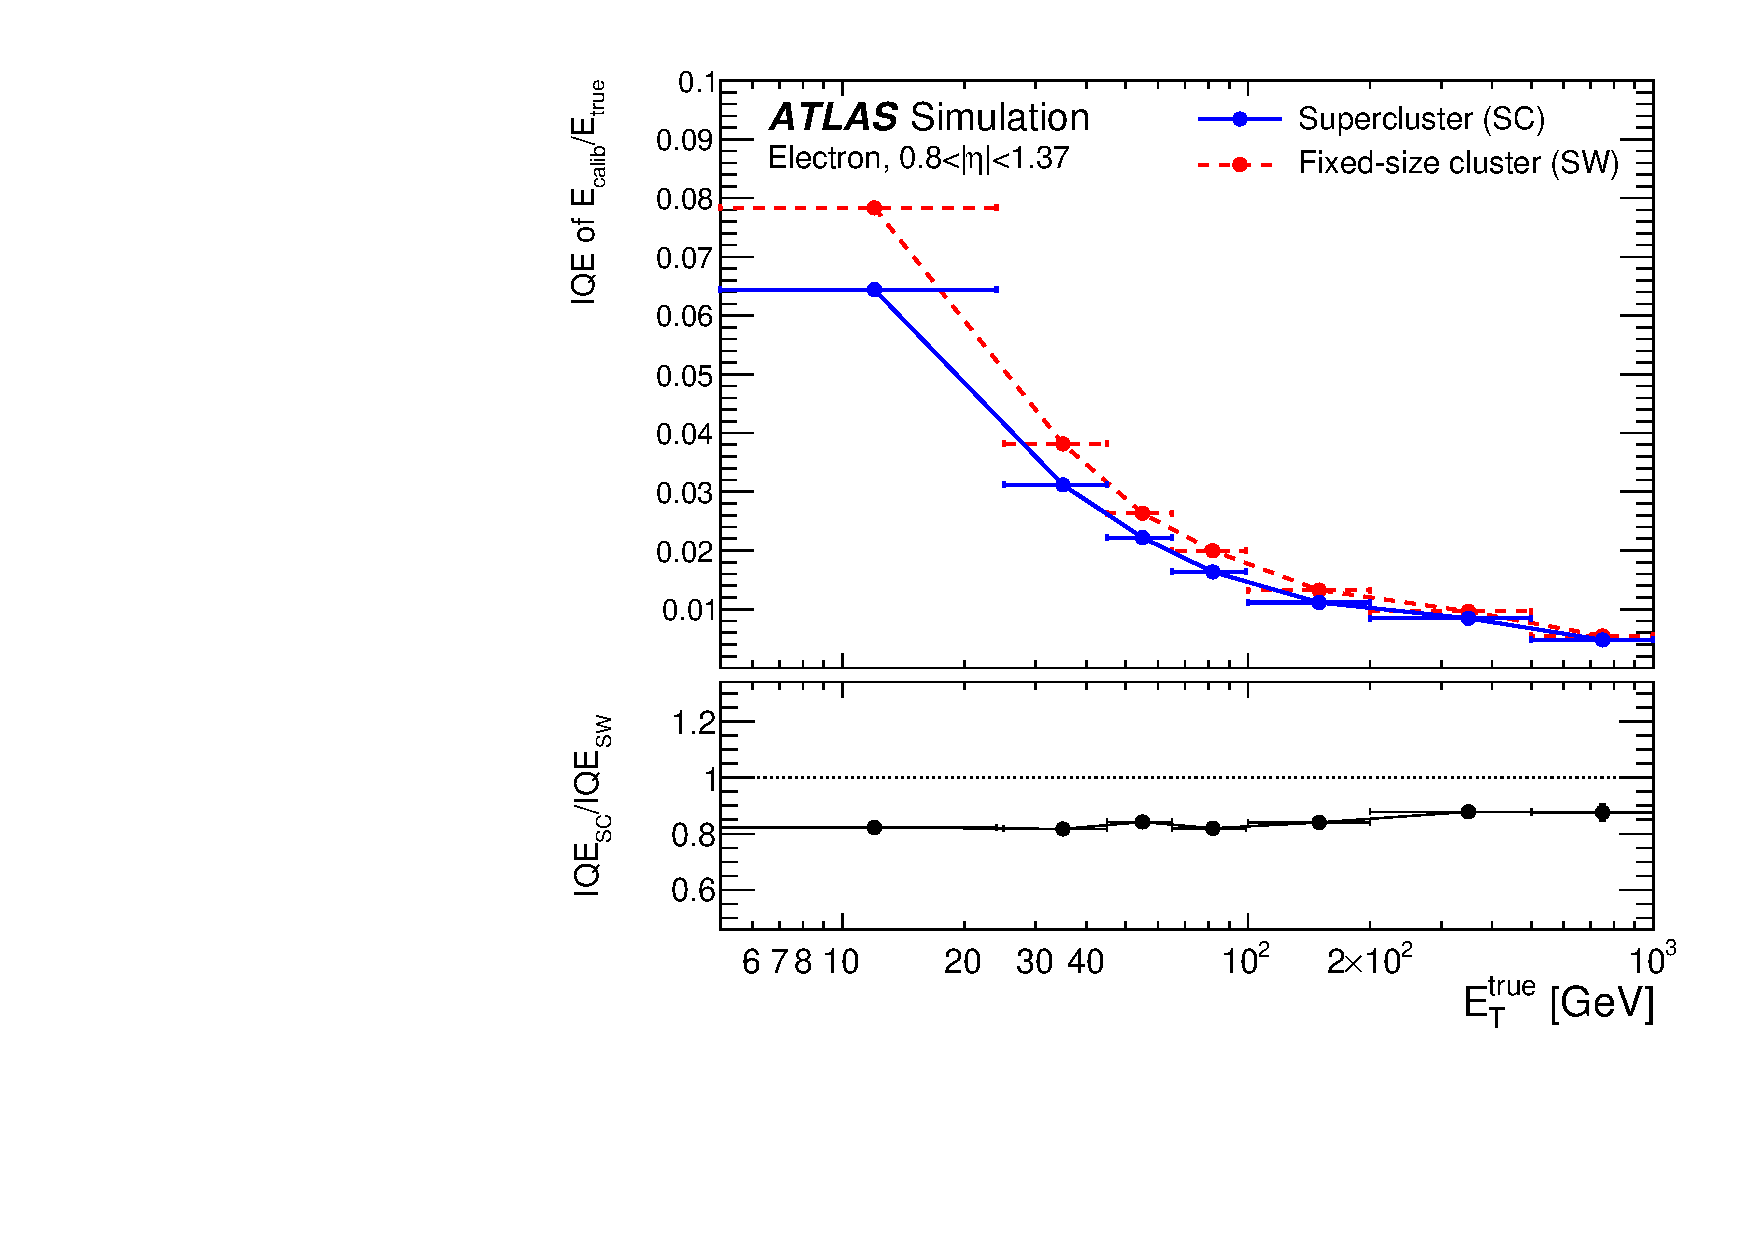
\includegraphics[width=\mediumfigwidth]{images/IQE_reco_1.pdf}
    \caption[Calibrated energy response resolution, expressed in terms of IQE, for simulated electrons]{Calibrated energy response resolution, expressed in terms of IQE, for simulated electrons. The response for fixed-size clusters based on the sliding window method is shown in dashed red, while the supercluster-based one is shown in full blue. The bottom panel shows the ratio between the supercluster-based algorithm and the sliding window algorithm~\cite{Aad:2019tso}.}
    \label{fig:method:iqe}
\end{figure}

\subsubsection{Electron identification}
Physics processes can \emph{fake} the prompt electron signature that can pass the reconstruction algorithms. Prompt electrons are defined as electrons which originate from the hard scattering vertex and are not the result of hadronic decays. Fake prompt electrons can arise from sources such as, hadronic showers which mimic an electron shower, and electrons from photon conversions. Non-prompt electrons can originate from the semileptonic decays of heavy-flavour hadrons.

Further criteria referred to as \emph{identification} is defined to select a sample of pure prompt electrons. A likelihood-based identification method is employed in the identification of prompt electrons. The method combines signal and background probability density functions of discriminating variables from quantities measured from the detector. These quantities include transition radiation in the TRT and shower shape in the EM calorimeter. An overall probability for an object to be constructed as an electron is calculated using the variables described above. The discriminating variable $d_\mathcal{L}$ is defined as
\begin{equation}
    d_{\mathcal{L}} = \frac{\mathcal{L}_S}{\mathcal{L}_S + \mathcal{L}_B},  
\end{equation}
with 
\begin{equation}
    \mathcal{L}_{S(B)}(\overrightarrow{x}) = \prod_{i=1}^{n} P_{i}^{S(B)} (x_{i}),
\end{equation}

where $\overrightarrow{x}$ is the vector of the n discriminating variables, $P_{i}^{S(B)}$ is the evaluation of the signal probability density function for the $i^{th}$ discriminating variable at the value $x_i$ under the signal (background) hypothesis. 

Three identification working points are defined for electron identification: \emph{loose}, \emph{medium} and \emph{tight}. Due to the non-exclusive nature of the working points, reconstructed electrons identified as tight also belong to the medium identification category, and electrons identified as medium belong to the loose identification category. The efficiencies of the identification working points are measured in data and simulation using $Z \rightarrow ee$ and $J/\psi \rightarrow ee$ decays in bins of $\abs{\eta}$ and $E_T$~\cite{Aad:2019tso}.~\cref{fig:method:reco:ideff} shows the efficiencies of the identification working points. These working points offer prompt electron identification efficiencies of 97\%, 95\% and 91\%, with background rejection efficiencies of 99.7\%, 99.8\% and 99.9\%, respectively. Even though the medium and tight efficiencies are lower compared to the loose criteria, the reduction in efficiency is accompanied by an increase in rejection of background processes by a factor of 2.0 and 3.5, respectively. The discontinuity in the efficiencies at $E_T = \SI{15}{\giga\electronvolt}$ is caused by a known mismodelling of the variables used in the likelihood discriminant at low $E_T$. 

\begin{figure}[]
    \centering
    \begin{subfigure}[b]{0.49\textwidth}
        \centering
        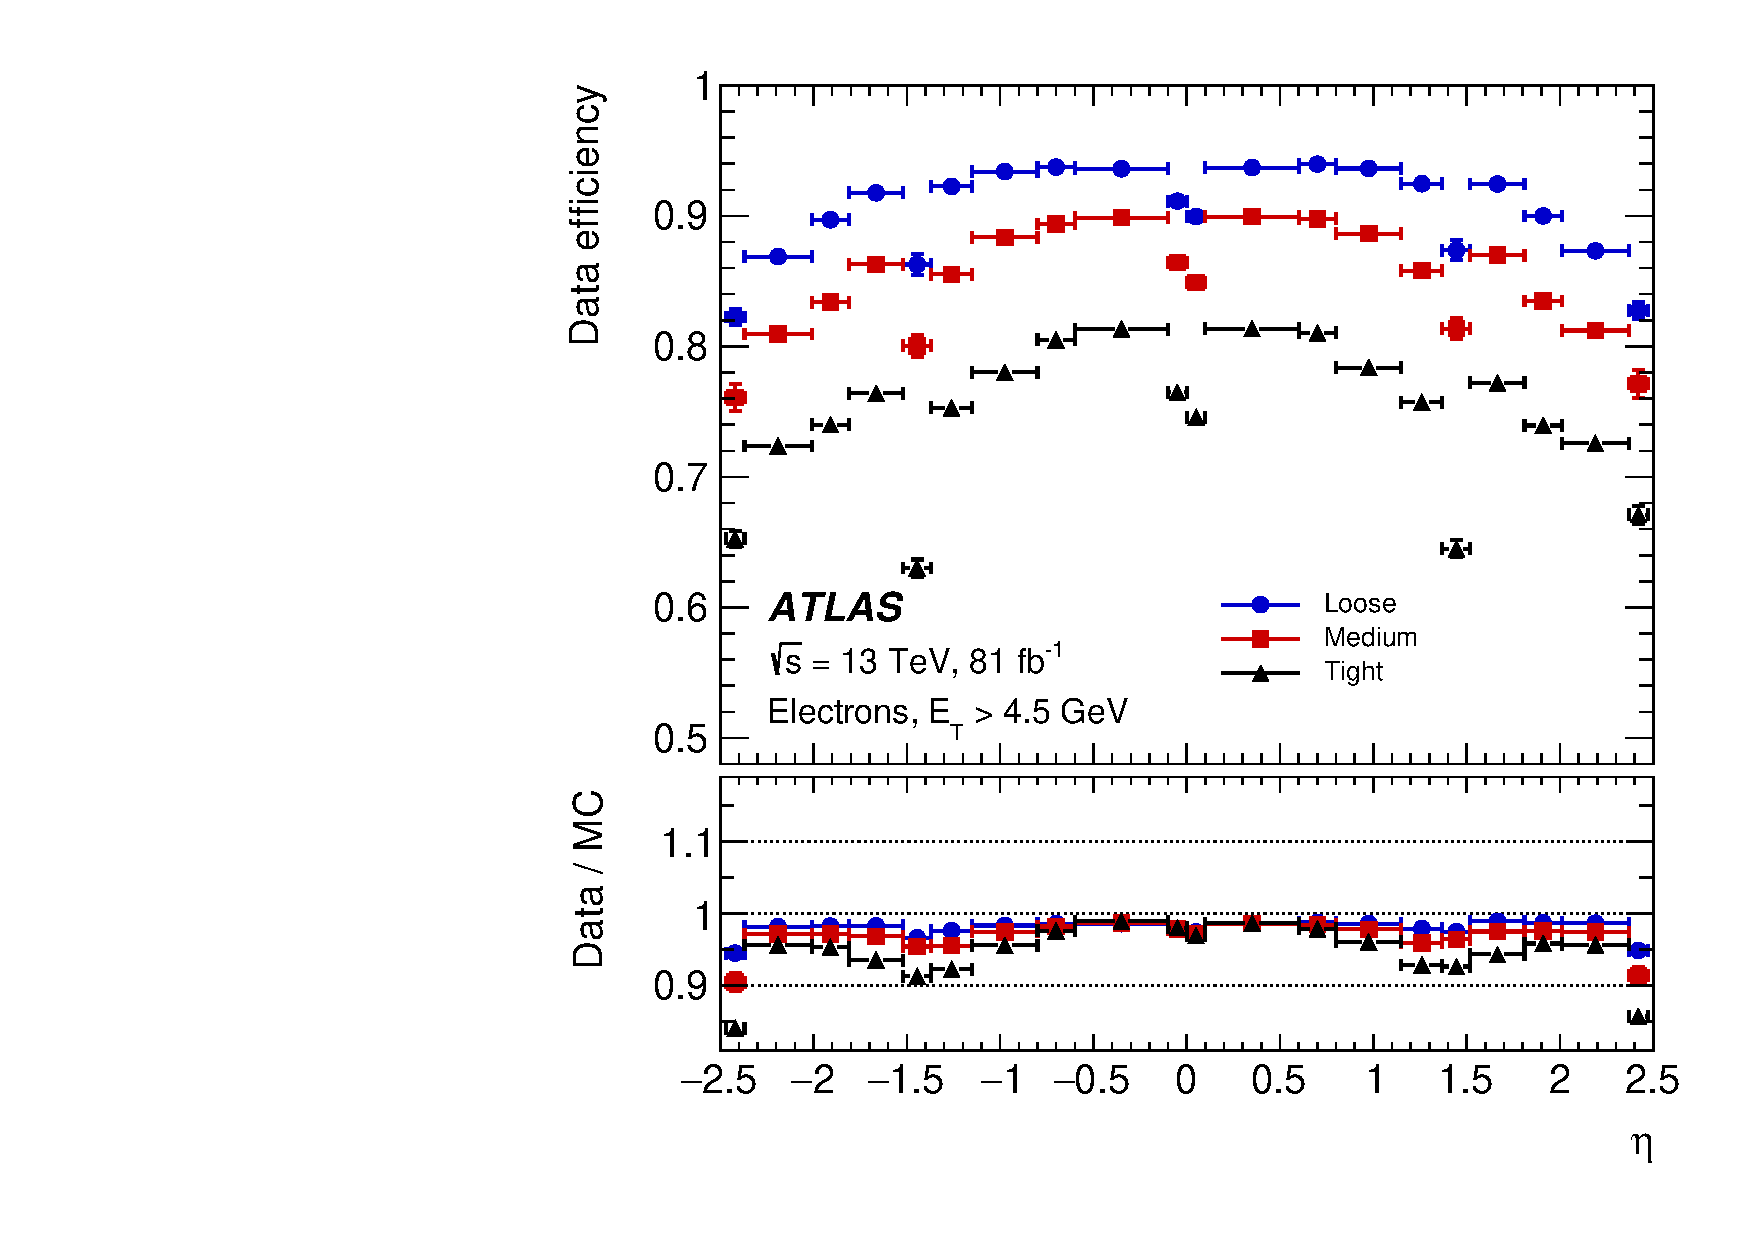
\includegraphics[width=\textwidth]{figures/reconstruction/figures_electronID_id_effeta.pdf}
        \caption{}
        \label{fig:method:reco:idetaeff}
    \end{subfigure}
    \begin{subfigure}[b]{0.49\textwidth}
        \centering
        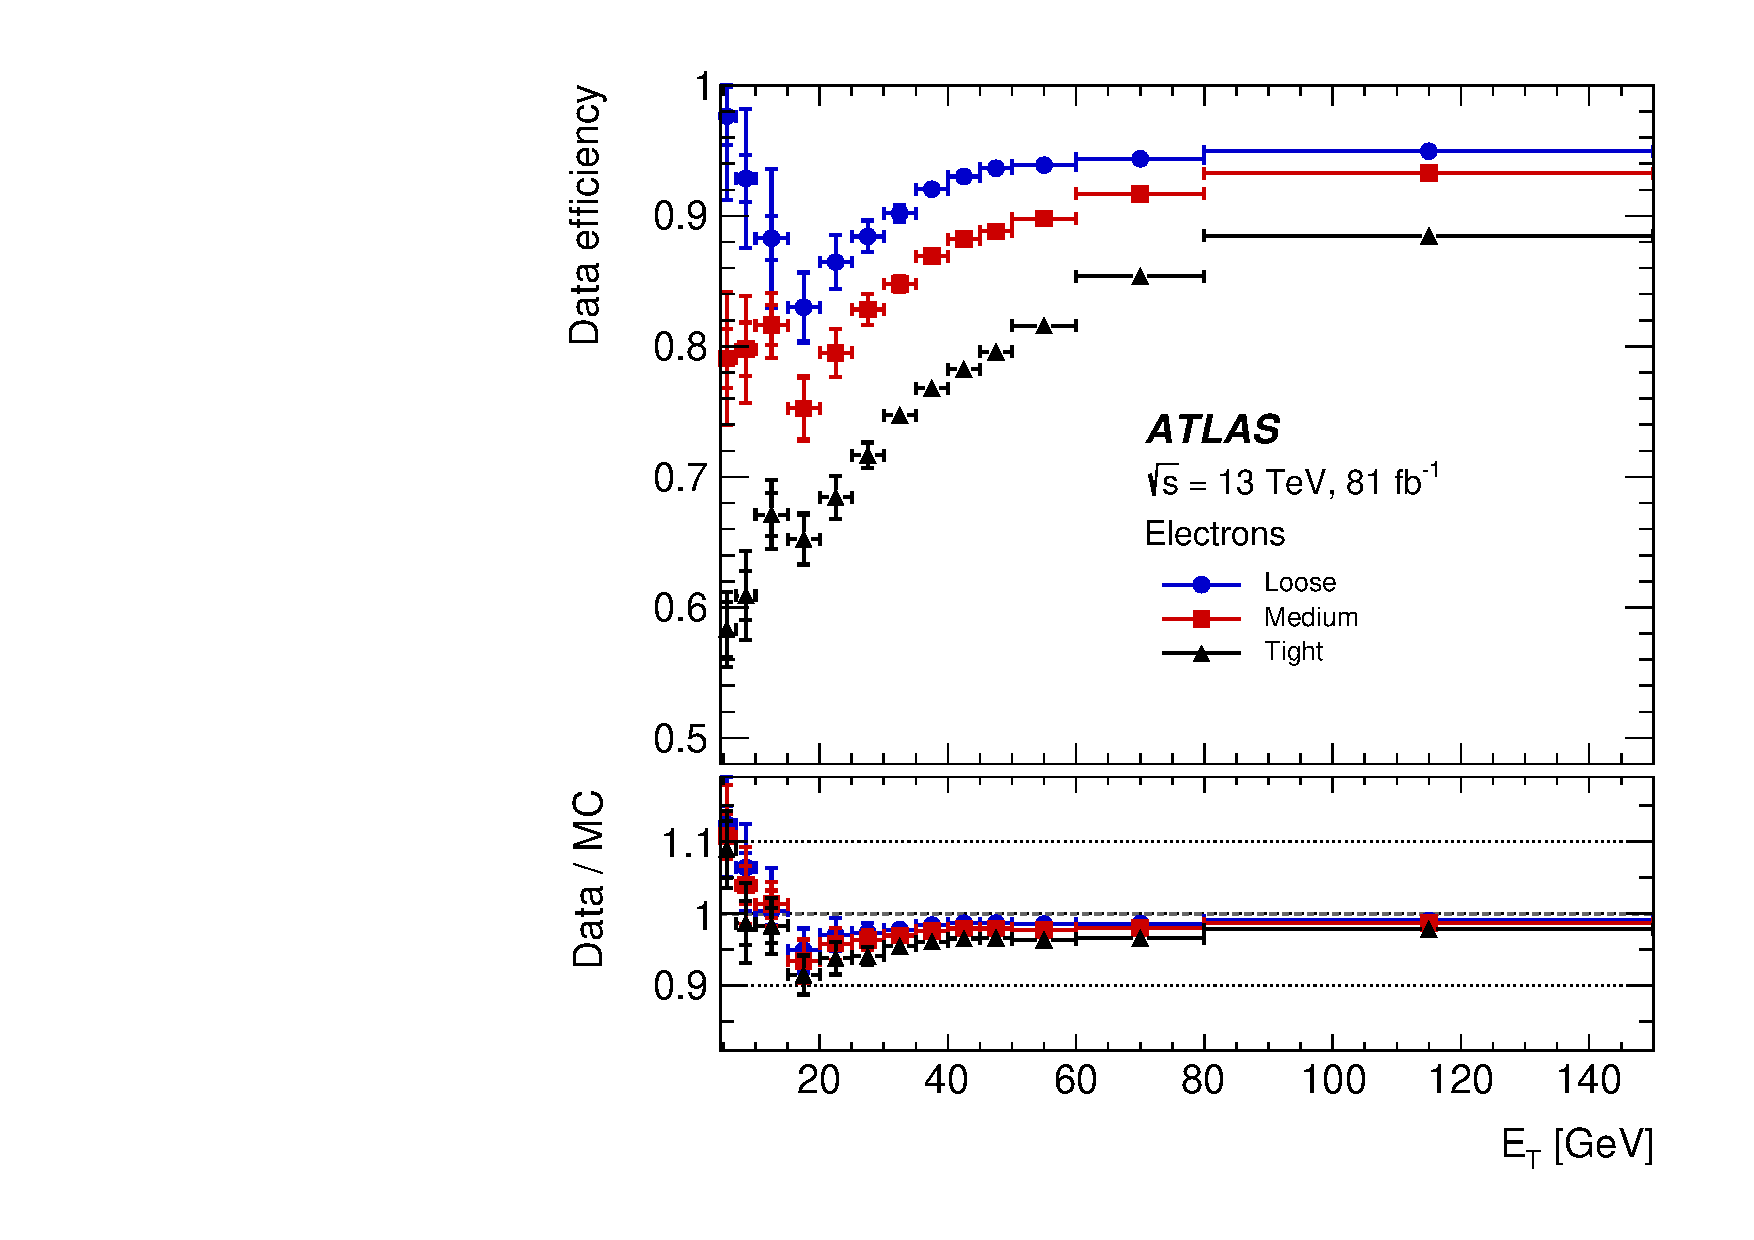
\includegraphics[width=\textwidth]{figures/reconstruction/figures_electronID_id_effpt.pdf}
        \caption{}
        \label{fig:method:reco:idpteff}
    \end{subfigure}
    \caption[Electron identification efficiency as a function of $\eta$ and as a function of $E_T$ for the identification working points]{Electron identification in data as a function of (a) $E_T$ and (b) $\eta$ for the loose, medium and tight identification working points. The inner uncertainties are the statistical. The total uncertainties are statistical and systematic uncertainties in the data-to-simulation efficiency ratio added in quadrature~\cite{Aad:2019tso}.}
    \label{fig:method:reco:ideff}
\end{figure}

\subsubsection{Electon isolation}
To further improve the purity of the prompt electron sample, and reject the background from hadronic decays, isolation requirements are applied based on the transverse energy around the electron candidate. Two types of isolation criteria are used: calorimeter and track-based isolation~\cite{Aad:2019tso}.

For the raw calorimeter isolation ($E_{T,\mathrm{raw}}^{\mathrm{isol}}$), the sum of the transverse energy of positive energy topo-clusters whose barycenter falls within a cone around the electron cluster is used. The raw EM particle energy ($E_{T,\mathrm{core}}$) is also contained within the cone and is required to be subtracted. This subtraction is done by removing the energy of EM calorimeter cells contained in a $\eta \times \phi = 5 \times 7$ around the EM particle cluster. Leakage corrections as a function of $\eta$ and $\phi$ are applied since the subtraction does not subtract all of the EM particle energy. A correction for the pileup and underlying-event contributions to the isolation cone is also estimated~\cite{Cacciari:2007fd}. The corrected calorimeter isolation variable is computed as
\begin{equation}
    E_{T}^{\mathrm{coneXX}} = E_{T,raw}^{\mathrm{isolXX}} - E_{T,\mathrm{core}} - E_{T,\mathrm{leakage}}(E_T,\eta,\Delta R) - E_{{T,\textrm{pile-up}}}(\eta,\Delta R),
\end{equation}
where XX refers to the size of the cone, $\Delta R = XX/100$. A cone size $\Delta R = 0.2$ is used for electron working points.  

The track isolation ($p_{T}^{\mathrm{coneXX}}$) is computed by summing the transverse momentum of selected tracks within a cone centered around the reconstructed electron track, excluding tracks matched to electron or converted photons. Track isolation for electrons is defined with a variable cone size ($p_{T}^{\mathrm{varconeXX}}$), which accounts for electrons produced in high-momentum particle decays where the decay products can be very close to the electron track. Therefore, the cone size gets smaller for larger transverse momentum, given by the equation: 
\begin{equation}
    \Delta R = \min \left( \frac{10}{p_T[\SI{}{\giga\electronvolt}]}, \Delta R_{\mathrm{max}}\right),
\end{equation}
where $\Delta R_{max}$ is maximum cone size, typically $\Delta R_{max} = 0.2$. 

The definitions of the different electron isolation working points are shown in~\cref{tab:ele_wps}. The working points result from a need for compromise between the efficiency of identification of prompt electrons and a good rejection of electrons from hadronic processes. The gradient working point is defined by a fixed value of efficiency designed to give an efficiency of 90\% at \pt = \SI{25}{\giga\electronvolt}, uniform in $\eta$. The three other working points have a fixed requirement on calorimeter and track isolation variables. The efficiencies for the electron isolation working points are shown on \cref{fig:method:reco:isoeleff}. The results are obtained using a sample enriched in $Z\rightarrow ee$ events. A jump in the efficiency for the gradient working point is observed at \SI{15}{\giga\electronvolt} due to the cut maps being optimised with $J/\Psi \rightarrow ee$ events below \SI{15}{\giga\electronvolt}, while the measurement is performed on $Z\rightarrow ee$ events in the full range. The tight working point gives the highest background rejection below \SI{60}{\giga\electronvolt}. The HighPtCaloOnly working point gives the highest rejection in the high-\et region ($\et > \SI{100}{\giga\electronvolt}$). For electrons with \et higher than \SI{500}{\giga\electronvolt} no measurement can be performed because of the limited number of data events. Therefore, the results from the \et bin [300,500]~\SI{}{\giga\electronvolt} are used with an additional systematic uncertainty varying between 0.1\% and 1.7\% depending on the isolation working point. 

\begin{table}[]
  \centering
  \resizebox{\textwidth}{!}{
  \begin{tabular}{lcc}
\hline \hline
    Working point & Calorimeter isolation  & Track isolation    \\ \hline

    Gradient         & $\epsilon=0.1143\times \pt+92.14\%$ (with \etcs)       & $\epsilon=0.1143\times \pt+92.14\%$ (with \ptvcs) \\ \hline
    HighPtCaloOnly & $\etcs < \text{max}(0.015\times \pt, 3.5~ \SI{}{\giga\electronvolt})$ & -                                                            \\
    Loose          & $\etcs/\pt < 0.20$                                     & $\ptvcs /\pt < 0.15$                \\
    Tight          & $\etcs/\pt < 0.06$                                     & $\ptvcs /\pt < 0.06$                \\
\hline
\hline
  \end{tabular}
  }
  \caption[Definition of the electron isolation working points and isolation efficiency $\epsilon$.]{Definition of the electron isolation working points and isolation efficiency $\epsilon$.
    In the Gradient working point definition, the unit of \pt is \SI{}{\giga\electronvolt}. All working points use a cone size
    of $\Delta R = 0.2$ for calorimeter isolation and $\Delta R_{\mathrm{max}} = 0.2$ for track isolation~\cite{Aad:2019tso}.}
  \label{tab:ele_wps}
\end{table}

\begin{figure}[]
    \centering
    \begin{subfigure}[b]{0.49\textwidth}
        \centering
        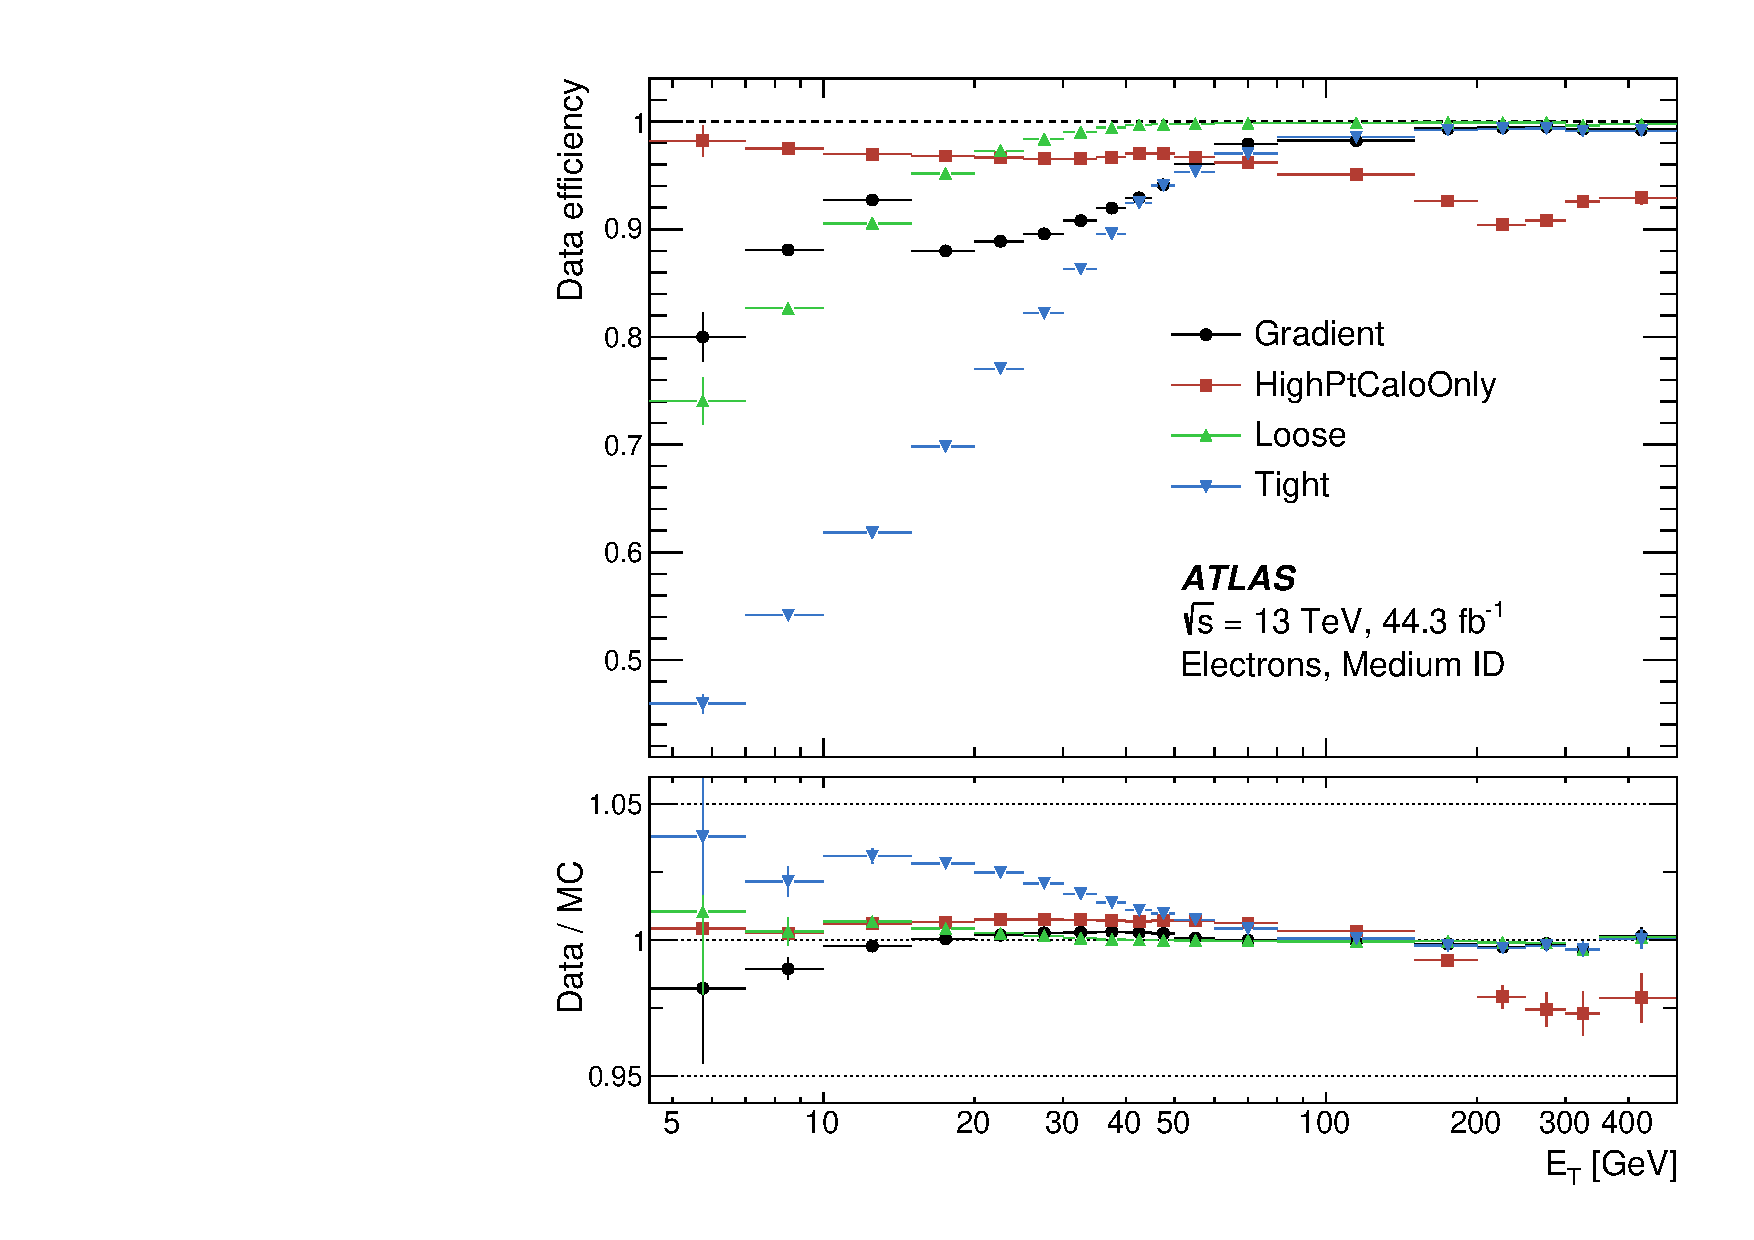
\includegraphics[width=\textwidth]{figures/reconstruction/figures_ele_iso_eff_sf_vs_pt_data17_MediumLH_4WPs.pdf}
        \caption{}
        \label{fig:method:reco:isoetaeff}
    \end{subfigure}
    \begin{subfigure}[b]{0.49\textwidth}
        \centering
        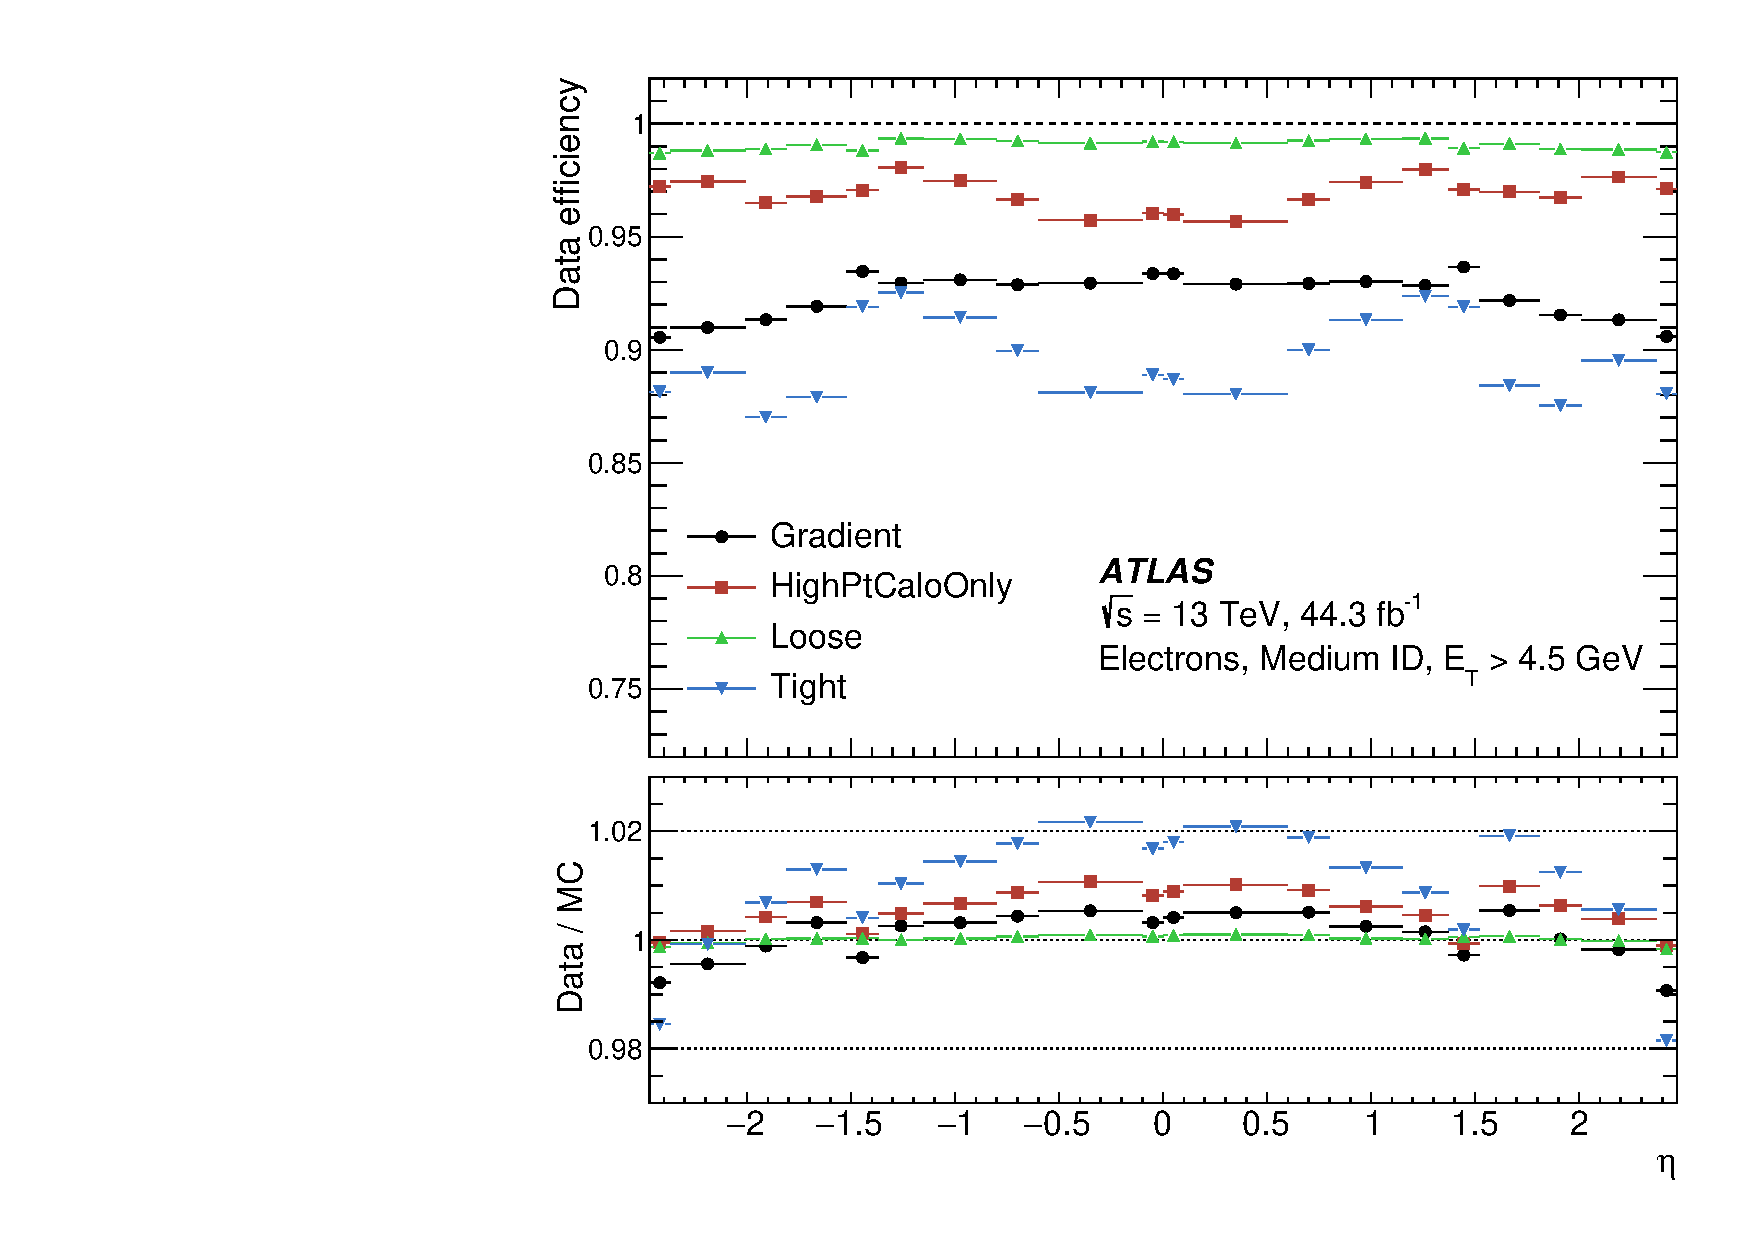
\includegraphics[width=\textwidth]{figures/reconstruction/figures_ele_iso_eff_sf_vs_eta_data17_MediumLH_4WPs.pdf}
        \caption{}
        \label{fig:method:reco:isopteff}
    \end{subfigure}
    \caption[Electron isolation efficiency as a function of $\eta$ and as a function of $E_T$ for the isolation working points]{Efficiency of the different isolation working points for electrons
    from inclusive $Z \rightarrow e^+e^-$ events as a function of the electron (a) $\et$ and
    (b) $\eta$. The electrons are required to fulfil the Medium selection from the likelihood-based electron identification. The lower panel shows the ratio of the efficiencies measured in data and in MC simulations. The total uncertainties are shown, including the statistical and systematic components~\cite{Aad:2019tso}.}
    \label{fig:method:reco:isoeleff}
\end{figure}

\subsection{Muons}\label{sec:reconstruction:muons}
Muon reconstruction is performed individually in the ID (described in~\cref{sec:reconstruction:tracks,sec:method:ID}) and muon spectrometer (described in \cref{sec:method:MS}). The information from these sub-detectors is then combined to form the muon tracks that are used in the thesis. Similar reconstruction criteria to electrons is also applied to the muon identification and isolation~\cite{Aad:2016jkr}. 

An important quantity in the reconstruction of muons in the ATLAS detector is its transverse momentum, defined as: 
\begin{equation}
    \pt = p\sin\theta = \frac{\sin\theta}{\abs{q/p}},
\end{equation}
where q/p is the ratio of the muon charge to its momentum and is measured from the track curvature. The muon track sagita, described in~\cref{sec:method:MS} is used when the muon tracks segments originate from all stations of the muon spectrometer. For muons with track segments in only two stations, the curvature is determined from the angular difference between the two segments. 

\subsubsection{Muon reconstruction}
Reconstruction of tracks in the muon spectrometer starts with the formation of segments found using search patterns inside each of muon spectrometer stations. In the MDT layers and the trigger chamber, a Hough transform~\cite{HoughTransform} is used to search for hits and a straight line fit is performed on the hits found in each layer. The RPC and TGC hits measure the coordinate orthogonal to the bending plane. Track segments in the CSC layers are built using a separate combinatorial search in the $\eta$ and $\phi$ planes~\cite{Aad:2016jkr}. 

The muon track candidates are then formed by fitting together the hits from segments in the different layers. Segments from the middle layers of the detector, where more hits are available, are used as seeds when the algorithm performs a combinatorial search. The search is then extended to use segments in the inner and outer layers as seeds. Several tracks can be built initially from the same segment. However, an overlap removal is later applied to select the best assignment to a single track, or it allows the segment to be shared between two tracks. A global $\chi^2$ fit is performed on the hits associated with each track. The track candidate is accepted if the $\chi^2$ satisfies the selection criteria. Hits providing a fit with a large $\chi^2$ are removed, and the track fit is repeated. Additional hits found to be consistent with the track candidate trajectory are added and then refit. 

Several algorithms are used to combine the muon track candidates in ID and muon spectrometer, where each algorithm uses different sets of information related to the detector components. Four main algorithms are used depending on the sub-detector used in the reconstruction:
\begin{itemize}
    \item \textbf{Combined (CB) Muon:} A global fit using the track candidates found in the ID and muon spectrometer is performed to form a CB muon. To improve the fit quality hits can either be added or removed from the track during the global fit. Most muons are first reconstructed in the muon spectrometer and then extrapolated inwards to the ID hits. Additionally, a complementary approach is utilised where the ID tracks are extrapolated outwards and matched to muon spectrometer hits. This approach accounts for a small fraction of the muons reconstructed. CB muons are the primary type used within ATLAS as they have the highest purity among the different classes of muons.
    \item \textbf{Segment-tagged (ST) Muons:}  An ID track is classified as a muon if, when extrapolated to the muon spectrometer, it is matched with at least one track segment in the MDT or CSC chambers. It has the lowest purity amount all classes of muons.
    \item \textbf{Calorimeter-tagged (CT) Muons:} Tracks in the ID are matched to energy deposits in the calorimeter compatible with a minimum ionising particle. 
    \item \textbf{Extrapolated (ME) Muons:} The muon trajectory is reconstructed from information based only on the muon spectrometer track and can be extrapolated to the interaction point, taking into account energy loss of the muons traversing through the calorimeters. 
\end{itemize}

An overlap removal procedure between the different types of muons is used, where if two types of muons share the same track, preference is given to CB, followed by ST, and then to CT muons. The overlap removal procedure for ME muons are performed by analysing the track hit content and selecting tracks with better fit quality. 

\subsubsection{Muon identification}
Muons which originate from decays of hadrons will have a characteristic deflection in their reconstructed tracks. This deflection will result in poor track quality and may not be compatible with the measured momentum in the ID and muon spectrometer. Several variables are selected to identify prompt muons. For CB tracks, the variables used in identification are:
\begin{itemize}
    \item \textbf{q/p significance:} The absolute difference between the charge and momentum ratio of the muons measured in the ID and MS divided by sum in quadrature of the uncertainties. 
    \item \textbf{$p^\prime$:} The absolute difference between the \pt measurements in the ID and muon spectrometer divided by the \pt of the combined track.
    \item $\chi^2$ of the fit.
\end{itemize}
In addition, requirements on the number of hits in the ID and muon spectrometer are also used. 

Four muon identification criteria are used to address the requirements of different physics analyses. The identification working points provided are: 
\begin{itemize}
    \item \textbf{Medium:} These are the default selection for ATLAS analysis. The selection minimises the systematic uncertainties associated with the reconstruction. CB muon tracks are required to have $\geq 3$ hits in at least two MDT layers (excluding $\abs{\eta} < 0,1$). ME tracks are required to have at least three MDT/CSC layers in the range $2.5 \geq \abs{\eta} \geq 2.7$. q/p significance is required to be less than seven.
    \item \textbf{Loose:} CB and ME muons satisfying the medium selection are included in the loose selection. Furthermore, CT and ST muons are restricted to the $\abs{\eta} < 0.1$ region.
    \item \textbf{Tight:} CB muons with hits in two stations and satisfying the medium selection are considered. Additionally, the normalised $\chi^2$ is required to be less than eight. Finally, a two dimensional cut on q/p significance and \emph{$p^\prime$} is also applied. 
    \item \textbf{High-\pt:} The High-\pt muon selection is used in the selection of muons in the analysis presented in this thesis. High-\pt muons are chosen to maximise the momentum resolution for tracks with \pt above \SI{100}{\giga\electronvolt} and is optimised for analyses that extend far into high \pt regions. CB muons which have at least three hits in at least three muon stations are selected. A veto is applied on muons with hits in specific regions of the muon spectrometer with suboptimal alignment. This procedure reduces the reconstruction efficiency by $20\%$, but improves the muon \pt resolution by $30\%$.
\end{itemize}

~\cref{tab:mm_ideff} shows the signal and background efficiencies of the different working points for muons in the range of $\SI{20}{\giga\electronvolt} < \pt < \SI{100}{\giga\electronvolt}$ obtained from $t\bar{t}$ simulation. An isolation requirement is not applied in the samples shown. When an isolation requirement is applied the misidentification rate is expected to be reduced by approximately an order of magnitude. 

\begin{table}[]
    \centering
    {
    \begin{tabular}{l||c|c||c|c}
  \hline \hline
      & \multicolumn{2}{c||}{$\SI{4}{\giga\electronvolt} \leq \pt \leq \SI{20}{\giga\electronvolt}$}  & \multicolumn{2}{c}{$\SI{20}{\giga\electronvolt} \leq \pt \leq \SI{100}{\giga\electronvolt}$ }    \\ 
      \hline \hline
      Selection & $\epsilon^{MC}_\mu$ [\%] & $\epsilon^{MC}_{Hadrons}$ [\%]& $\epsilon^{MC}_\mu$ [\%]& $\epsilon^{MC}_{Hadrons} $[\%] \\
      \hline
      Loose & 96.7 & 0.53 & 98.1 & 0.76 \\ 
      Medium & 95.5 & 0.38 & 96.1 & 0.17 \\
      Tight & 89.9 & 0.19 & 91.8 & 0.11 \\
      High-\pt & 78.1 & 0.26 & 80.4 & 0.13 \\
  \hline
  \hline
    \end{tabular}
    }
    \caption[Efficiency for prompt muons from $W$ decays and hadrons decays misidentified as prompt muons]{Efficiency for prompt muons from W decays and hadrons decays misidentified as prompt muons computed using a $t\bar{t}$ MC sample. The results are shown for the four identification selection criteria separating low and high momentum for muon candidates~\cite{Aad:2016jkr}.}
    \label{tab:mm_ideff}
  \end{table}

\subsubsection{Muon isolation}
Similar to electrons, isolation criteria are also applied on muon candidates to improve background rejection. Three isolation variables are defined to asses the muon isolation: two track-based and a calorimeter-based isolation variable:
\begin{itemize}
    \item Variable track-based $p_{T}^{varcone30}$: Defined as the sum of transverse momentum of tracks in a cone of $\Delta R = min(\SI{10}{\giga\electronvolt}/p_{T}^{\mu},0.3)$ with $\pt > \SI{1}{\giga\electronvolt}$, around the candidate muon track. 
    \item Fixed track-based $p_{T}^{cone20}$: Defined as the sum of the transverse momentum of all tracks within a cone of $\Delta R = 0.2$ around the candidate muon track.
    \item Calorimeter based $\et^{cone20}$: Defined as the sum of the transverse momentum of all topological clusters within a cone of $\Delta R = 0.2$ from the candidate muon. 
\end{itemize}

Several isolation working points are available depending on the needs of the analysis. In many isolation working point a ratio of the isolation variable and the muon \pt is used to improve the efficiency over the full \pt spectrum. For the analysis discussed in this thesis, the \emph{FCTightTrackOnly} isolation is used, which requires $\pt^{varcone30}/\pt < 0.6$. 

% \subsubsection{Correction factors}

% Scale factors are applied to electrons and muons from simulated events to ensure consistency with the efficiency of the electrons and muons found in data. A total scale factor is applied correcting for mismodelling in tracking and shower shapes, and electron energy scale, reconstruction and selection efficiencies.

\subsection{Jets}

\subsubsection{Jet reconstruction}
Jets are collimated showers of particles produced from the hadronisation of gluons emerging from proton-proton collisions, resulting in energy deposits in the calorimeters. Their energy is deposited in the hadronic calorimeters distinguishing them from electrons or photons. There are various algorithms available for jet reconstruction~\cite{Atkin_2015}. The ATLAS experiment focuses on the \emph{anti-$k_\text{T}$} algorithm~\cite{antikt}, where topo-clusters are built from calorimeter cells as input. The \emph{anti-$k_T$} algorithm calculates distances between every pair of inputs $i$ and $j$ as:
\begin{equation}
    d_{ij} = \min\!\left(k_{ti}^{2p}, k_{tj}^{2p}\right) \frac{\Delta^2_{ij}}{R^2}, 
\end{equation}
with the distance to the beam axis,
\begin{equation}
    d_{iB} = k_{ti}^{-2}.
\end{equation}
where $\Delta_{ij} = (y_i - y_j)^2 - (\phi_i - \phi_j)^2$, $k_{ti}$, $y_i$ and $\phi_i$ are the transverse momentum, rapidity and azimuthal angle of particle i, respectively. The jet radius parameter $R$ can vary depending on the analysis using the algorithm and is typically set to $\Delta R = 0.4$. 

For each set of inputs, the algorithm compares the distances $d_{ij}~\mathrm{and}~d_{iB}$. If $d_{ij} < d_{iB}$ then the four-momenta of the input \emph{j} is combined with input \emph{i}. If, $d_{ij} > d_{iB}$, then $i$ is declared a final jet and removed from the list of entities. The algorithm terminates when the list of entries is empty and all of the inputs have been classified. 

% \subsubsection{b-jets}
% \emph{b-jets} are a class of jet that are the result of decays of \emph{b} quarks. The \emph{b} quarks hadronise to \emph{B} hadrons. The b-jets travel for longer distances within the detector, on the order of several millimetres, compared to other types of jets. Therefore, experimental techniques can be used to \emph{tag} the jets containing \emph{B} hadrons~\cite{ATLAS:PHYS-PUB-2015-022,ATLAS:PHYS-PUB-2016-012}.

\subsection{Missing transverse momentum}
Weakly interacting particles (e.g. neutrinos) can traverse through the ATLAS detector without interacting with any of the detector material. Therefore, they cannot be reconstructed. This leaves a characteristic missing transverse momentum signature in the detector defined as: 
\begin{equation}
   \et^{miss} = - \left[ ~\sum^{\mathrm{all ~objects}}_i \pt^i + \et^{cl}~ \right],
\end{equation}
where the summation includes the transverses momentum $\pt^i$ of all leptons, jets and photons. $\et^{cl}$ accounts for all energy clusters in the calorimeters that are not associated with a reconstructed object~\cite{ATL-PHYS-PUB-2015-027}.

\clearpage